\def\difficulty{1}
\sujet{Harris corner detector}
\index{Features!Harris Corner Detector}
\begin{note}The aim of this tutorial is to develop a simple Harris corner detector. This is the first step in pattern matching, generally followed by a feature descriptor construction, and a matching process.\end{note}

\vspace*{-10pt}

\section{Corner detector and cornerness measure}

\vspace*{-10pt}

\begin{mcomment}
\begin{mremark}
 Use \minline{imgradientxy} and \minline{imgaussfilt} with a scale parameter $\sigma$ that will constrain the size of the window $W$.
\end{mremark}
\end{mcomment}

\begin{pcomment}
\begin{premark}
 Use the \pinline{sobel} and \pinline{gaussian_filter} from the \pinline{scipy.ndimage} module.
\end{premark}
\end{pcomment}

\vspace*{-3pt}

\subsection{Gradient evaluation}

The Harris corner detector is based on the gradients of the image, $I_x$ and $I_y$ in x and y directions, respectively.

\begin{qbox}
 Apply a Sobel gradient in both directions in order to compute $I_x$ and $I_y$.
\end{qbox}


\subsection{Structure tensor}
The structure tensor is defined by the following matrix. The coefficients $\omega$ follow a gaussian law, and each summation represents a gaussian filtering process. $W$ is an operating window.\vspace*{-7pt}
\[
M=
\begin{bmatrix}
\underset{(u,v)\in W}\sum \omega(u,v) I_x(u,v)^2 &\underset{(u,v)\in W} \sum \omega(u,v) I_x(u,v) I_y(u,v) \\
\underset{(u,v)\in W}\sum \omega(u,v) I_x(u,v) I_y(u,v) & \underset{(u,v)\in W}\sum \omega(u,v) I_y(u,v)^2
\end{bmatrix} =
\begin{bmatrix}
M_1 & M_2 \\
M_3 & M_4
\end{bmatrix}\vspace*{-8pt}
\]

\begin{qbox}
 \begin{itemize}
  \item Evaluate $M_1$ to $M_4$ for each pixel of the image.
 \end{itemize}

\end{qbox}

\vspace*{-2pt}

\subsection{Cornerness measure}
The cornerness measure $C$, as proposed by Harris and Stephens, is defined as follows for every pixel of coordinates $(x,y)$:\vspace*{-8pt}
\[ 
C(x,y) = \textrm{det}(M)-K \textrm{trace}(M)^2\vspace*{-8pt}
\]
with $K$ between 0.04 and 0.15.

\begin{qbox}
 Compute $C$ for all pixels and display it for several scales $\sigma$.
\end{qbox}

\section{Corners detection}
A so-called Harris corner is the result of keeping only local maxima above a certain threshold value.  You can use the checkerboard image for testing, or load the sweden road sign image Fig.\ref{fig:harrs:enonce:road_sign}.

\begin{mcomment}Use the command \minline{checkerboard(8)>.5} for generating a checkerboard figure, or load the road sign:
	\begin{matlab}
		I = imread('sweden_road.png');
	\end{matlab}
\end{mcomment}

\begin{pcomment}
	
Use the following function to generate a checkerboard pattern.	
\begin{python}
def checkerboard(nb_x=2, nb_y=2, s=10):
	"""
	checkerboard generation
	a grid of size 2*nb_x by 2*nb_y is generated
	each square has s pixels.
	"""
	C = 255*np.kron([[1, 0] * nb_x, [0, 1] * nb_x] * nb_y, np.ones((s, s)))
	return C
\end{python}
	
\end{pcomment}


\begin{figure}[H]
\centering\caption{Sweden road sign to be used for corner detection.}%
 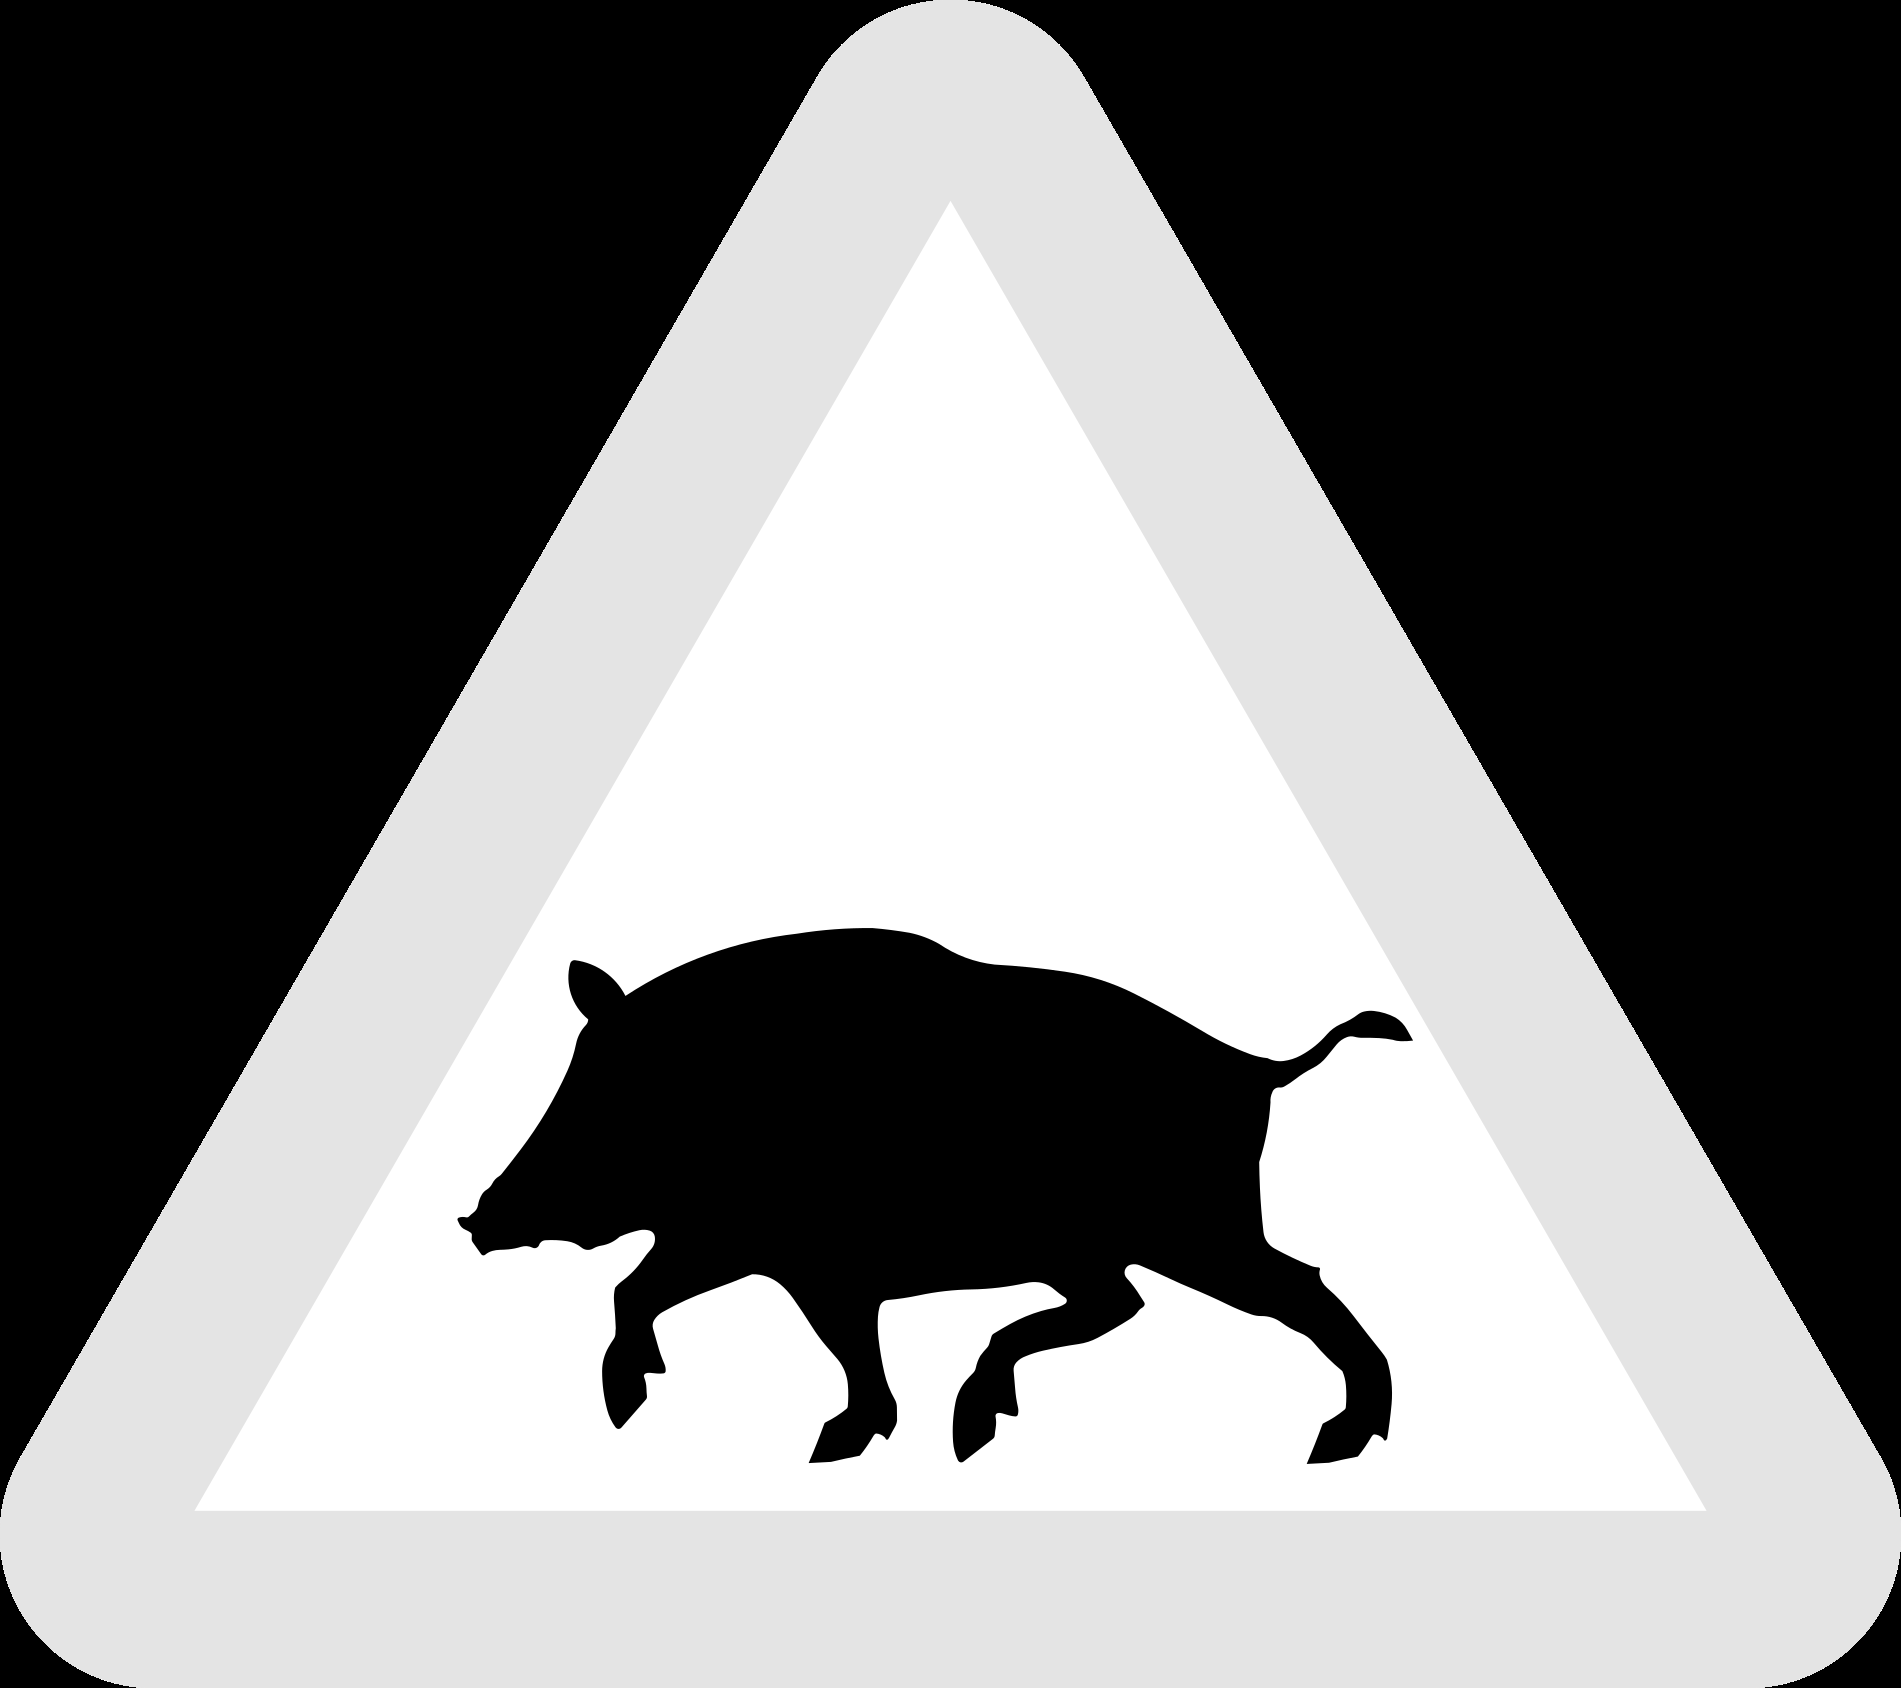
\includegraphics[width=5cm]{sweden_road.png}%
 \label{fig:harrs:enonce:road_sign}%
\end{figure}



\begin{qbox}
 \begin{itemize}
 \item Evaluate the extended maxima of the image.
 \item Only the strongest values of the cornerness measure should be kept. Two strategies can be employed in conjonction:
 \begin{itemize}\item Use a threshold value $t$ on $C$: the choice of this value is not trivial, and it strongly depends on the considered image. An adaptive method would be preferred.
 \item Keep only the $n$ strongest values.
 \end{itemize}
  \item The previous operations are affected by the borders of the image. Thus, eliminate the corner points near the borders.
  \item The detected corners may contain several pixels. Keep only the centroid of each cluster.
  
 \end{itemize}

\end{qbox}
